\section{Realios mašinos projektas}

\subsection{Techninės įrangos komponentai}

\begin{figure}[H]
  \begin{center}
    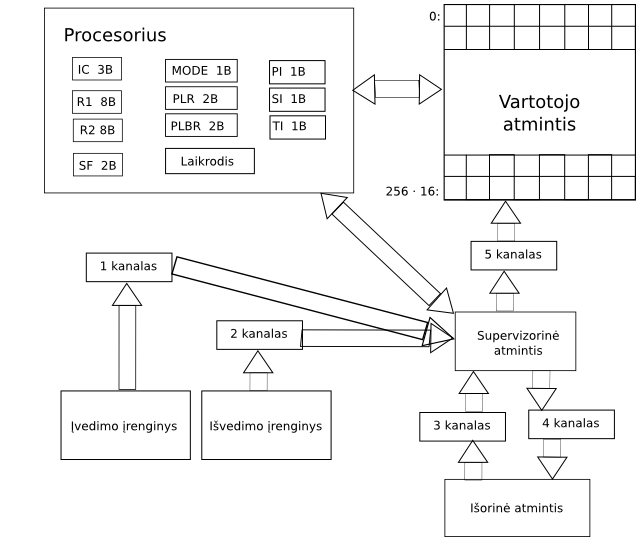
\includegraphics[width=1.0\linewidth]{rm.png}
  \end{center}
  \caption{Realios mašinos architektūra.}
  \label{fig:rm}
\end{figure}
% TODO Patikrinti ar schema atitinka reikalavimus.

\begin{description}
  \item[Procesorius] gali dirbti dviem rėžimais: naudotojo ir 
    supervizoriaus. Naudotojo rėžime vykdomos virtualios mašinos komandos,
    o supervizoriaus rėžime – operacinės sistemos. Laiko tarpas, per
    kurį procesorius atlieka vieną komandą laikomas vienu laiko vienetu.
    Procesorius turi šiuos registrus:
    \begin{description}
      \item[$IC$] 3 baitų nuorodos registras. Skirtas nurodyti vykdomos 
        virtualios mašinos komandos adresą atmintyje.
      \item[$R1$] 8 baitų bendro naudojimo registras.
      \item[$R2$] 8 baitų bendro naudojimo registras.
      \item[$PLR$] 2 baitų nuorodų registras. Skirtas nurodyti puslapių 
        lentelės bloko adresą.
      \item[$PLBR$] 2 baitų nuorodų registras. Skirtas nurodyti puslapių 
        lentelės pirmojo baito vietą \verb|PLR| bloke.
      \item[$MODE$] 1 baito loginis registras, kurio reikšmė nusako 
        procesoriaus darbo rėžimą („N“ – naudotojas, „S“ – supervizorius).
      \item[$SF$] 2 baitų loginis registras, skirtas saugoti aritmetinių 
        operacijų loginių (teisinga „1“ arba klaidinga „0“) reikšmių sekai. 
        Lentelėje pateikta informacija apie logines reikšmes:

        \begin{tabularx}{0.85\textwidth}{|c|c|c|X|}
          \hline
          Bitas & Trumpinys & Reikšmė & Paaiškinimas %& C++ funkcija 
          \\
          \hline
          0 & CF & pernešimo požymis & įgija „1“ tada, kai sudėties arba
          atimties rezultatas netelpa į žodį 
          %& \verb|((bool) ((sk1+sk2) & (1<<8)))| 
          \\
         %\hline
         %2 & PF & lyginumo požymis & & 
         %\verb|!((bitset<8>(sk1+sk2).count())&1)| \\
         %\hline
         %4 & AF & papildomo pernešimo požymis & 
         %  \verb|((bool) (((sk1&0xff)| 
         %  \verb|+ (sk2&0xff))&(1<<4)))| \\
          \hline
          6 & ZF & nulio požymis & parodo ar paskutinės operacijos 
          rezultatas yra nulinis %& \verb|(!(sk1+sk2))| 
          \\
          \hline
          7 & SF & ženklo požymis & parodo, koks yra paskutinės operacijos 
          rezultato ženklas („1“ – jei neigiamas) 
          %& \verb|((bool) ((sk1+sk2) & (1<<7)))| 
          \\
         %\hline
         %8 & TF & „spąstų“ požymis & jei „1“, tai po kiekvienos komandos
         %įvyksta pertraukimas & \\
         %9 & IF & & \\
         %10 & DF & & \\
          \hline
          11 & OF & perpildymo požymis & įgija „1“ tada, kai rezultatas
          netelpa skaičių su ženklu diapazone arba mėginama atlikti 
          aritmetines operacijas su neteisingo formato argumentais.
          %& \verb|(((sk1&(1<<7))==(sk2&(1<<7)))&&|
          %  \verb|((sk1&(1<<7))==((sk1+sk2)&(1<<7))))| 
          \\
          \hline
        \end{tabularx}
      \item[$PI$] 1 baito registras programiniams pertraukimams fiksuoti.
        (Pavyzdžiui, buvo aptiktas neegzistuojantis operacijos kodas, ar
        adresas „išeina“ už numatytų ribų.)
      \item[$SI$] 1 baito registras supervizoriniams pertraukimams fiksuoti.
        (Supervizorinis pertraukimas įvyksta tada, kai virtuali mašina
        pati negali atlikti veiksmo (pavyzdžiui, darbas su įvedimu ir
        išvedimu) ir ji kreipiasi į operacinės sistemos servisą.)
      \item[$TI$] 1 baito registras laikrodžio pertraukimams fiksuoti.
      \item[$IOI$] 1 baito įvedimo / išvedimo pertraukimo registras – 
        praneša, kad veiksmas baigėsi. Kadangi vienu 
        metu gali įvykti keli pertraukimai, tai $i$-ojo kanalo pertraukimas
        fiksuojamas prie registro reikšmės pridedant $2^{i-1}$.
      \item[$CHST$] 1 baito kanalų užimtumo registras. Nurodoma, jog
        $i$-asis kanalas užimtas prie registro reikšmės pridedant 
        $2^{i-1}$.
    \end{description}

    Taip pat procesoriuje yra laikrodis – laiko matavimo įrenginys, kuris
    vienodais laiko intervalais generuoja pertraukimus. 

    Procesorius dirba su simboliniais duomenimis bei sveikaisiais 
    skaičiais su ženklu, užrašytais simboliniu formatu.
  \item[Vartotojo atmintis] yra atmintis skirta virtualių mašinų atmintims 
    bei puslapių lentelėms laikyti. Jos dydis 256 blokai po 16 žodžių, kur
    žodžio ilgis yra 8 baitai. Atmintis numeruojama nuo 0. Visi VM 
    puslapiai yra užkraunami prieš pradedant VM darbą.

    Pirmieji 16 blokų yra rezervuoti puslapiavimo mechanizmui. Registru
    \verb|PLR| nurodoma, kuriame bloke yra saugoma lentelė, o registru
    \verb|PLBR| nurodoma, kuriuo baitu bloke prasideda puslapių lentelė.
    Atminties baite, kurio pozicija yra $PLR \cdot 16 + PLBR$ ir po jo 
    esančiame baite yra saugoma, kiek blokų užima kodo segmentas 
    (pažymėkime $C (1 \leq C)$). Kitoje baitų poroje nurodyta kiek blokų 
    užima duomenų segmentas (pažymėkime $D (0 \leq D)$). Toliau yra 
    $C$ baitų porų, kuriose nurodyta kokie blokai atitinka kodo puslapius.
    Analogiškai, po jų yra $D$ baitų porų, kurie nurodo kokie blokai 
    atitinka, kuriuos duomenų puslapius. Toliau yra 36 baitai skirti
    informacijai apie atidarytus failus saugoti. Vienu metu gali
    būti atidaryti ne daugiau nei 4 failai. $i$-oji 9 baitų eilė yra skirtas
    informacijai apie atidarytą failą kurio $id$ yra $i$ saugoti. Jei
    pirmojo eilės baito reikšmė yra $0$, tai reiškia, kad failas nėra
    atidarytas. Jei jo reikšmė yra $i$, tai reiškia, jog failas yra
    įvedimo įrenginio abstrakcija, o jei $o$, tai kad išvedimo įrenginio.
    Jei $r$, tai failas yra atidarytas skaitymui ir like 8 baitai yra
    atidaryto failo pavadinimas. Analogiškai $w$ žymi failą atidarytą
    rašymui.

    Kiti 240 blokų yra skirti virtualių mašinų duomenims. 
    Inicijuojant virtualią mašina, kiekvienam jos reikalaujamam atminties
    puslapiui ieškomas blokas nuo viršaus.
  \item[Supervizorinė atmintis] jos dydis 16 blokų.
  \item[Išorinė atmintis] tai tiesioginio įėjimo ir išėjimo išorinis
    įrenginys, kuriame duomenys sugrupuoti į failus (failo pavadinimas
    yra mašinos žodis). Reali mašina gali failą sukurti, atidaryti
    skaitymui, atidaryti rašymui (atidarius failą rašymui, visa 
    jame buvusi informacija yra ištrinama) ir ištrinti. Iš failo skaitoma
    ir į jį rašoma 1 bloko dydžio ilgio įrašais. (Vienas apsikeitimas 
    trunka tris laiko vienetus.)
  \item[Duomenų perdavimo kanalai] yra 5. 
    \begin{description}
      \item[1 kanalu] perduodami duomenys iš įvedimo įrenginio į 
        supervizorinę atmintį.
      \item[2 kanalu] perduodami duomenys iš supervizorinės atminties
        į išvedimo įrenginį.
      \item[3 kanalu] perduodami duomenys iš kietojo disko į supervizorinę
        atmintį.
      \item[4 kanalu] perduodami duomenys iš supervizorinės atminties į 
        kietąjį diską.
      \item[5 kanalu] perduodami duomenys iš supervizorinės atminties į 
        vartotojo atmintį.
    \end{description}
  \item[Įvedimo ir išvedimo įrenginiai.] RM turi vieną nuoseklų įvedimo
    įrenginį ir vieną nuoseklų išvedimo įrenginį. Tiek duomenų nuskaitymas,
    tiek jų įrašymas vyksta fiksuoto 1 bloko dydžio įrašais. (Duomenų
    apsikeitimas su šiais įrenginiais trunka tris laiko vienetus.)
\end{description}
